\documentclass[11pt]{article}

\usepackage[margin=1in]{geometry}
\usepackage[T1]{fontenc}
\usepackage{lmodern}
\usepackage{microtype}
\usepackage{amsmath,amssymb,amsthm,mathtools}
\usepackage{graphicx}
\usepackage[dvipsnames]{xcolor}
\usepackage{booktabs}
\usepackage{hyperref}

\hypersetup{
  colorlinks=true,
  linkcolor=MidnightBlue,
  citecolor=MidnightBlue,
  urlcolor=MidnightBlue
}

\newtheorem{theorem}{Theorem}
\newtheorem{proposition}{Proposition}
\newtheorem{remark}{Remark}

\newcommand{\E}{\mathbb{E}}
\newcommand{\V}{\mathcal{V}}

\title{\textbf{Eliminative Information in a Generalized Monty Hall Problem IV}\\
\large Multiple Prizes with Unequal Rewards}
\author{}
\date{}

\begin{document}
\maketitle

\begin{abstract}
Parts I--III developed the generalized Monty Hall problem from identical prizes,
to variable reveal costs, to heterogeneous rewards and labeled priors. This
note isolates the intermediate case of multiple prizes with unequal values.
There are $K$ doors, exactly $m\ge1$ prize doors, and prize values
$v_1,\dots,v_m$, which need not be equal. We first study the exchangeable
model in which the multiset $\{v_1,\dots,v_m,0,\dots,0\}$ is placed uniformly
at random among door labels. In that case, unequal rewards still collapse to a
single scalar, the total reward mass
\[
  V=\sum_{i=1}^m v_i.
\]
Under uniform switching after $t$ zero reveals, expected stay value is $V/K$
and expected switch value is $V(K-1)/[K(K-1-t)]$. Thus unequal prizes alone do
not destroy the one-dimensional structure. The real complexity appears only
when door labels carry prior information or when switching ceases to be
uniform. We formulate the exchangeable theorem, derive the constant-cost
threshold, and supplement the theorem with empirical evidence in two stages:
Stage 1 verifies the exchangeable collapse numerically, while Stage 2 shows how
label-specific priors break that scalar picture and make initial choice,
switching rule, and Monty's policy strategically relevant.
\end{abstract}

\section{Setup}

There are $K$ doors, with $1\le m<K$ prize doors. Prize door $i$ carries value
$v_i>0$, and the remaining $K-m$ doors carry value $0$. Let
\[
  V=\sum_{i=1}^m v_i.
\]
We assume throughout that Monty knows realized prize locations and reveals only
zero-value doors, never opening the player's initial door.

The player:
\begin{itemize}
\item chooses one door initially;
\item observes $t$ zero-value reveals, with
\[
  0\le t\le K-m-1;
\]
\item then either stays, or switches to one of the remaining unopened
non-initial doors.
\end{itemize}

The main question is: how much of the Part I and Part III structure survives
when there are \emph{multiple prizes with unequal values}?

\section{Two Distinct Models}

As in Part III, the first split is conceptual.

\paragraph{Exchangeable unequal prizes.}
The multiset
\[
  \{v_1,\dots,v_m,0,\dots,0\}
\]
is placed uniformly at random among the $K$ door labels. Door labels carry no
prior information.

\paragraph{Labeled unequal prizes.}
Door labels have distinct priors over reward, so the identity of the initial
choice and the identity of Monty's reveals matter.

This note focuses first on the exchangeable case, because it is the cleanest
and pins down what unequal prizes do \emph{not} change.

\section{Exchangeable Unequal Prizes}

Assume the values $v_1,\dots,v_m$ are fixed, but their placement among the $K$
doors is uniform over labels. The player chooses an initial door uniformly.
Monty reveals $t$ zero-value doors. The player then switches uniformly among
the remaining unopened non-initial doors.

\begin{theorem}[Collapse to total reward mass]
Under exchangeable placement and uniform switching,
\[
  \E[\text{stay reward}]=\frac{V}{K}
\]
and
\[
  \E[\text{switch reward after }t\text{ reveals}]
  =
  \frac{V(K-1)}{K(K-1-t)}.
\]
\end{theorem}

\begin{proof}
By exchangeability, every door has the same ex ante expected reward. Since the
sum of rewards over all doors is $V$, the expected reward of the initial door is
$V/K$.

The expected reward mass outside the initial door is therefore
\[
  V-\frac{V}{K}=\frac{V(K-1)}{K}.
\]
Monty reveals only zero-value doors, so this expected outside reward mass is not
altered by the reveals. After $t$ reveals, the remaining non-initial closed set
has size $K-1-t$, and symmetry implies that uniform switching spreads this
outside reward mass evenly across those switch targets. Hence
\[
  \E[\text{switch reward after }t\text{ reveals}]
  =
  \frac{1}{K-1-t}\cdot\frac{V(K-1)}{K}
  =
  \frac{V(K-1)}{K(K-1-t)}.
\]
\end{proof}

\begin{remark}
If all positive prizes are unit prizes, then $V=m$, and this reduces exactly to
Part I:
\[
  \E[\text{stay}]=\frac{m}{K},
  \qquad
  \E[\text{switch after }t]=\frac{m(K-1)}{K(K-1-t)}.
\]
So unequal prize values do not change the exchangeable theory except through the
single scalar $V$.
\end{remark}

\section{Advantage of Switching}

The switch advantage in the exchangeable unequal-prize model is
\[
  \frac{V(K-1)}{K(K-1-t)}-\frac{V}{K}
  =
  \frac{Vt}{K(K-1-t)}.
\]
Thus the sign and comparative statics are exactly the same as in Part I:
\begin{itemize}
\item the switch advantage is nonnegative and strictly positive for $t>0$;
\item the gain from switching increases with reveal depth;
\item unequal prize values merely rescale the payoff level by $V$.
\end{itemize}

This makes the exchangeable unequal-prize model mathematically neat, but not yet
qualitatively new.

\section{Constant Reveal Costs}

Suppose each reveal costs a constant amount $c$. Then the net switch value
after $t$ reveals is
\[
  W(t)=\frac{V(K-1)}{K(K-1-t)}-ct.
\]
Its one-step increment is
\[
  \Delta_t=W(t+1)-W(t)
  =
  \frac{V(K-1)}{K(K-2-t)(K-1-t)}-c.
\]
Because the benefit term is increasing in $t$, the same endpoint logic as in
Part I survives. In particular, the comparison between full reveal and no
reveal is
\[
  \frac{V(K-1)}{Km}-c(K-m-1)
  \quad\text{versus}\quad
  \frac{V}{K}.
\]
This yields the critical constant-cost threshold
\[
  c^*=\frac{V}{Km}.
\]

\begin{remark}
When all prizes are unit prizes, $V=m$, so the threshold becomes
\[
  c^*=\frac{1}{K},
\]
recovering Part I exactly.
\end{remark}

\section{Stage 1 Empirical Evidence}

Stage 1 coding verifies that the exchangeable unequal-prize theorem is not just
a symbolic rescaling. The simulation draws explicit prize vectors, places them
uniformly among doors, reveals only legal zero doors, and estimates both stay
and switch values from Monte Carlo runs.

For the baseline experiment, we fix $K=12$, $m=4$, and use the unequal prize
vector $(1,2,5,9)$, so $V=17$. Figure~\ref{fig:theory-empirical} compares
the empirical estimates against the exact formulas over all feasible reveal
depths $t=0,1,\dots,K-m-1$. The agreement is close throughout. In the current
Stage 1 run, the largest absolute stay error is about $0.017$ and the largest
absolute switch error is about $0.037$, both well within ordinary Monte Carlo
noise for a finite simulation of this size.

\begin{figure}[t]
  \centering
  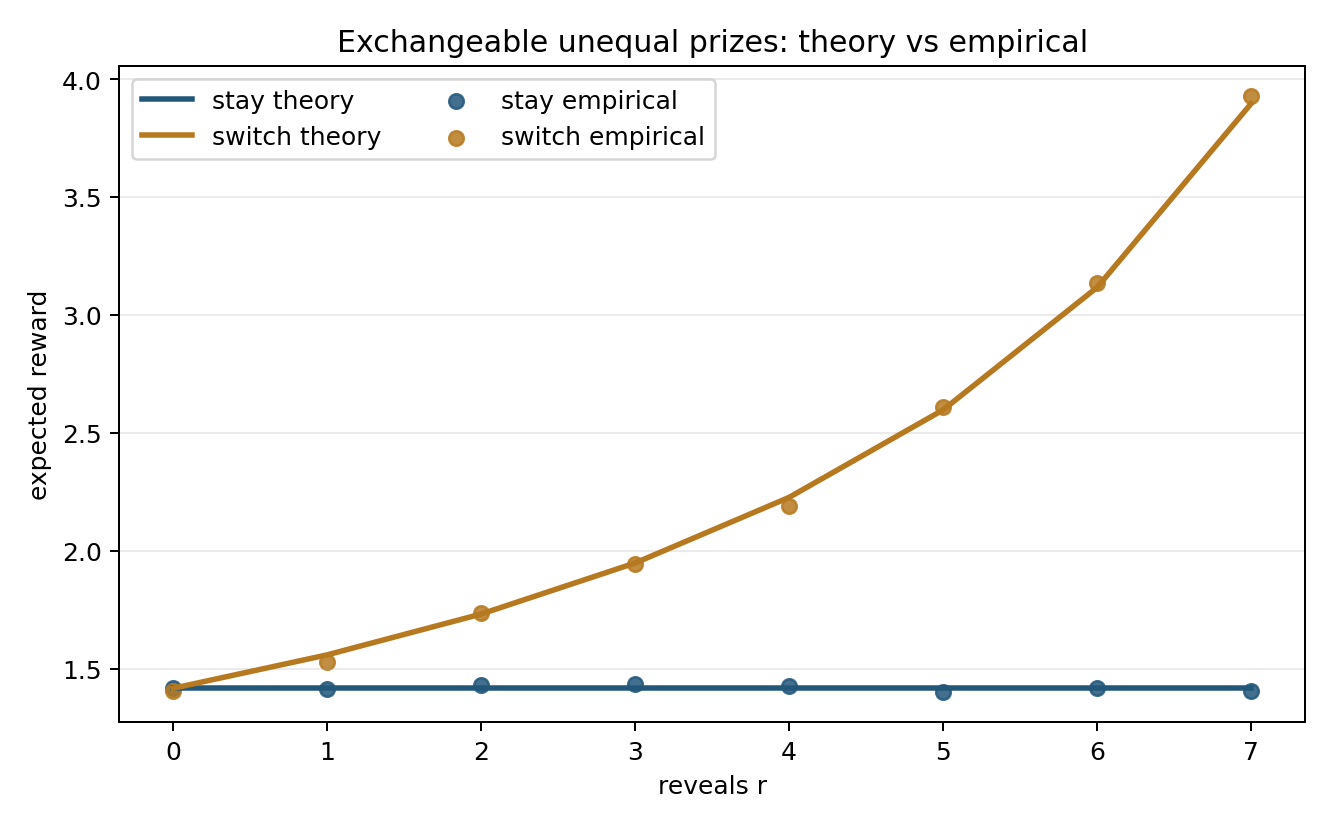
\includegraphics[width=0.92\linewidth]{../outputs/stage1_exchangeable_theory_vs_empirical.png}
  \caption{Stage 1 baseline verification for $K=12$, $m=4$, and reward vector
  $(1,2,5,9)$. Stay value is flat at $V/K$, while switch value rises with
  reveal depth exactly as predicted by $V(K-1)/[K(K-1-t)]$. The empirical
  points track the theoretical curves closely.}
  \label{fig:theory-empirical}
\end{figure}

The more important question is whether the collapse to total reward mass $V$ can
be seen directly in simulation when the prize vector itself changes shape.
Stage 1 therefore compares three distinct reward vectors,
\[
  (1,2,5,9),\qquad (4,4,4,5),\qquad (8,4,3,2),
\]
all of which satisfy $V=17$. These vectors differ substantially in how reward
mass is distributed across the $m=4$ prize doors, but under the exchangeable
model they should produce the same expected stay and switch values.

Figure~\ref{fig:same-v-collapse} shows exactly that. When plotted in raw reward
units, the empirical curves for same-$V$ reward vectors lie nearly on top of one
another, and they all follow the same theoretical shape. Figure~\ref{fig:normalized-collapse}
then divides reward by total mass $V$, making the scale-free claim visually
explicit: after normalization, the curves collapse onto the same geometry.

\begin{figure}[t]
  \centering
  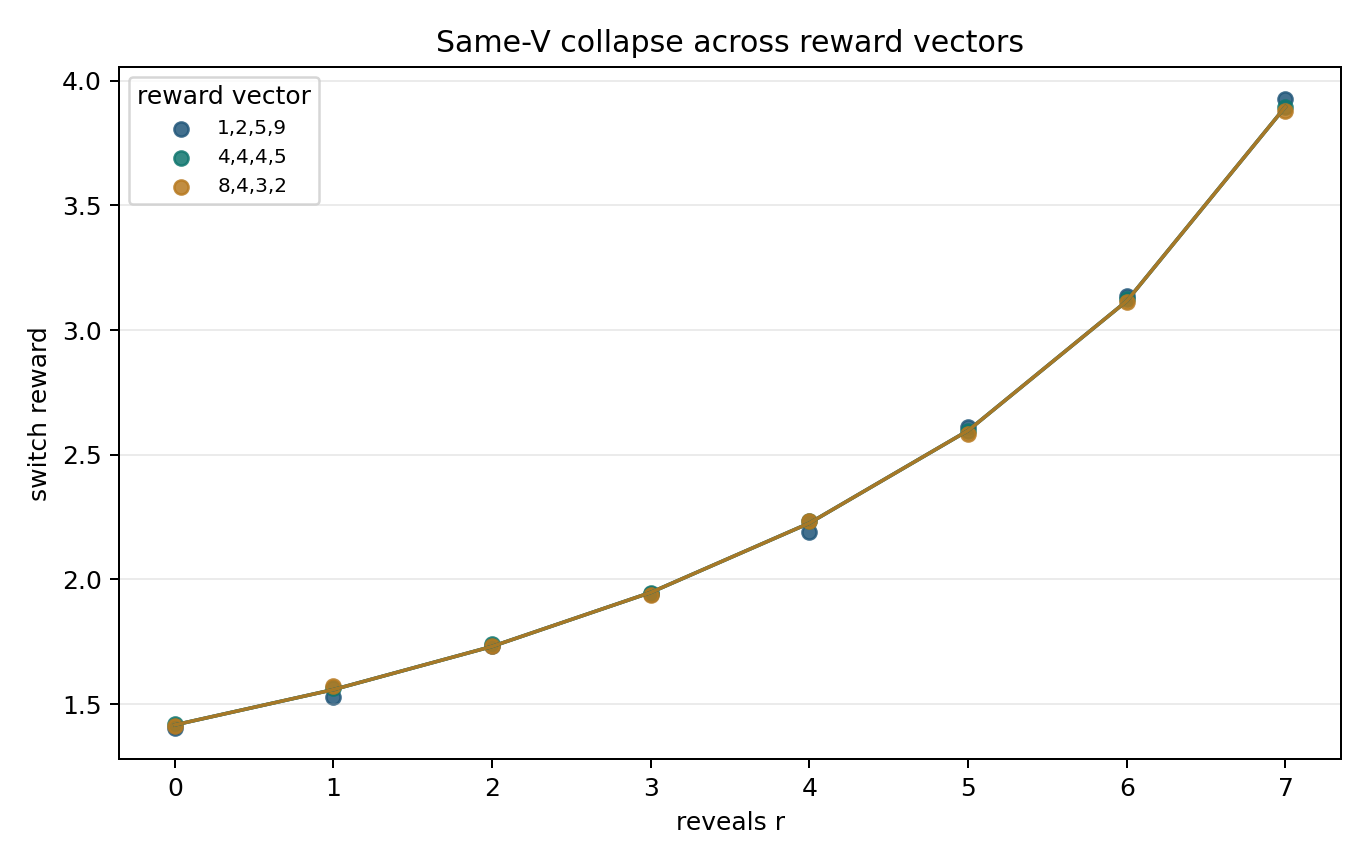
\includegraphics[width=0.92\linewidth]{../outputs/stage1_exchangeable_same_v_collapse.png}
  \caption{Same-$V$ collapse in raw reward units. Three distinct unequal prize
  vectors with the same total mass $V=17$ produce nearly identical empirical
  stay and switch curves across reveal depth.}
  \label{fig:same-v-collapse}
\end{figure}

\begin{figure}[t]
  \centering
  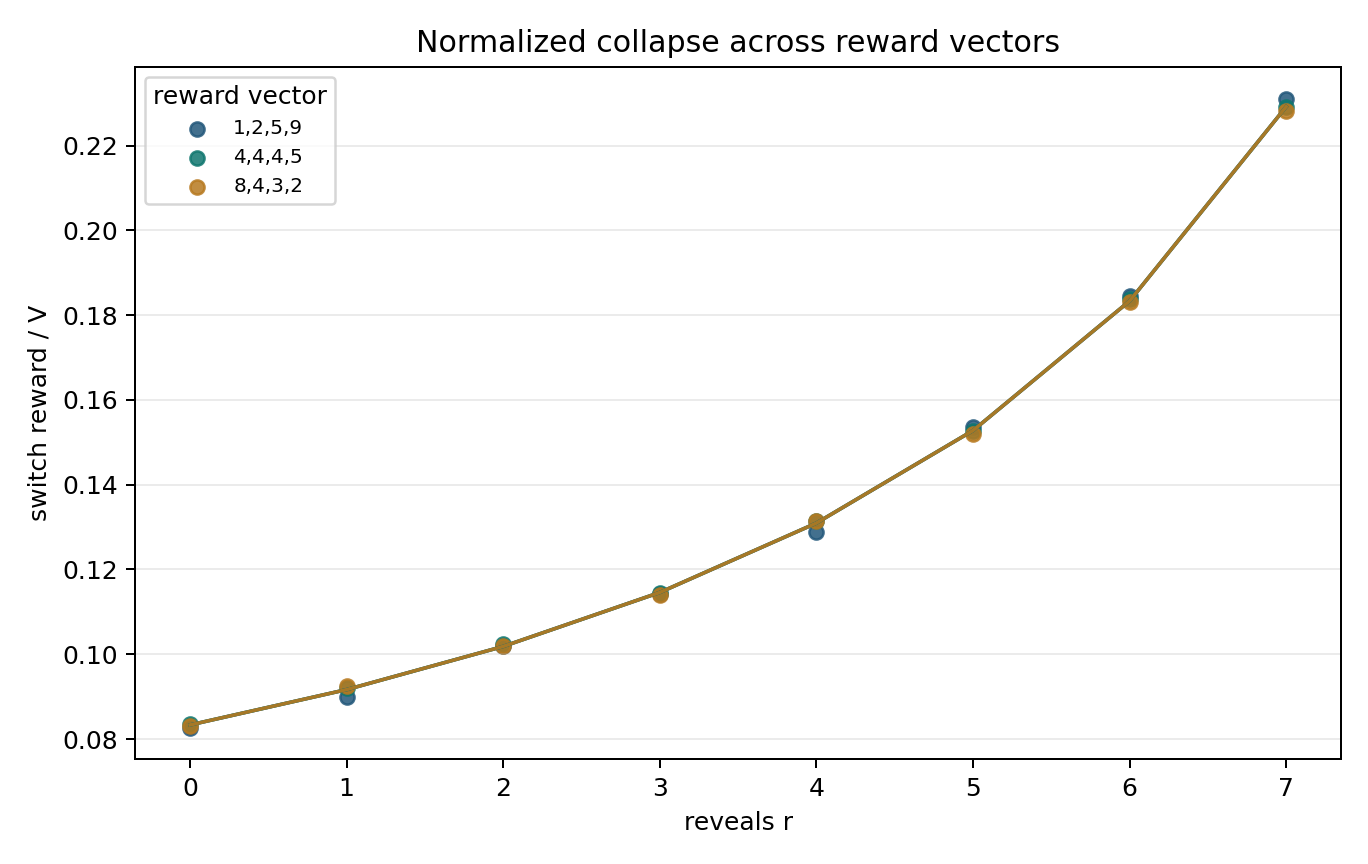
\includegraphics[width=0.92\linewidth]{../outputs/stage1_exchangeable_normalized_collapse.png}
  \caption{Normalized collapse after dividing by total reward mass $V$. This is
  the clearest empirical expression of the theorem: once values are normalized
  by $V$, the exchangeable unequal-prize model has the same reveal-depth
  geometry regardless of how the positive reward mass is partitioned among the
  $m$ prize doors.}
  \label{fig:normalized-collapse}
\end{figure}

These plots matter because they rule out a tempting but false intuition. One
might suspect that a ``spikier'' prize vector such as $(1,2,5,9)$ should behave
differently from a flatter vector such as $(4,4,4,5)$ even in the exchangeable
case. Stage 1 shows that this is not so. As long as labels are uninformative and
switching is uniform, the simulation respects the theorem: only total reward
mass matters.

\section{What Unequal Prizes Do Not Yet Change}

The exchangeable unequal-prize model leaves the problem essentially
one-dimensional. The relevant state variable is still just the reveal count
$t$, because label symmetry survives. The consequences are:
\begin{itemize}
\item stay and switch values depend only on total reward mass $V$;
\item the exact success-law geometry from Part I survives after a scalar
rescaling;
\item the variable-cost analysis from Part II also carries over with $m$
replaced by $V$ in the relevant payoff scale;
\item there is still no strategic initial choice, because all door labels are
ex ante equivalent.
\end{itemize}

So unequal prizes by themselves do \emph{not} create a new decision theory.
They create a new payoff scale.

\section{Where the Genuinely New Problem Begins}

The interesting Part IV problem is therefore not merely ``multiple prizes with
unequal rewards.'' It is:
\begin{quote}
multiple unequal rewards \emph{with labeled prior information over doors}.
\end{quote}

Once labels matter, the state ceases to be scalar. The player must track a
posterior reward landscape over remaining doors. Then:
\begin{itemize}
\item the initial door can again become strategic;
\item different switch rules no longer coincide;
\item Monty's reveal policy can carry value-relevant information;
\item multiple prize values create a richer posterior allocation problem than in
Part III.
\end{itemize}

A natural first labeled model is:
\[
  X_j\in\{0,v_j\}
\]
with
\[
  \mathbb{P}(X_j=v_j)=p_j,
  \qquad
  \mathbb{P}(X_j=0)=1-p_j,
\]
so each door has prior mean
\[
  \mu_j=p_jv_j.
\]
This is the direct multiple-prize unequal-value analogue of the Bernoulli-value
model from Part III.

\section{Stage 2: Labeled Unequal Prizes}

Stage 2 moves from exchangeable reward placement to explicit labeled priors. The
point is no longer to verify a scalar collapse theorem, because there is no such
scalar collapse left. Instead the goal is to expose which strategic dimensions
become relevant once door labels carry information.

The labeled model used in the code is:
\[
  X_j=
  \begin{cases}
    v_j & \text{with probability } p_j,\\
    0   & \text{with probability } 1-p_j.
  \end{cases}
\]
So each door has prior mean
\[
  \mu_j=p_jv_j.
\]
This model supports three initial strategies (`random', `highest\_mu',
`lowest\_mu'), three Monty policies (`uniform\_zero', `low\_mu\_zero',
`high\_mu\_zero'), and four switch rules (`stay', `uniform\_switch',
`prior\_best\_switch', `oracle\_best\_switch').

\subsection{A canonical skewed prior landscape}

For the first Stage 2 experiment, we use the explicit door priors
\[
  (p_j,v_j)\in\{(0.1,1),\ (0.2,1.5),\ (0.8,4),\ (0.3,2),\ (0.05,10)\}.
\]
The resulting prior means are
\[
  \mu=(0.1,\ 0.3,\ 3.2,\ 0.6,\ 0.5).
\]
Figure~\ref{fig:stage2-prior-landscape} shows this landscape directly. There is
one very strong prior-best door, several middling alternatives, and one
rare-but-large reward door. This is the sort of structure where label
information can plausibly matter.

\begin{figure}[t]
  \centering
  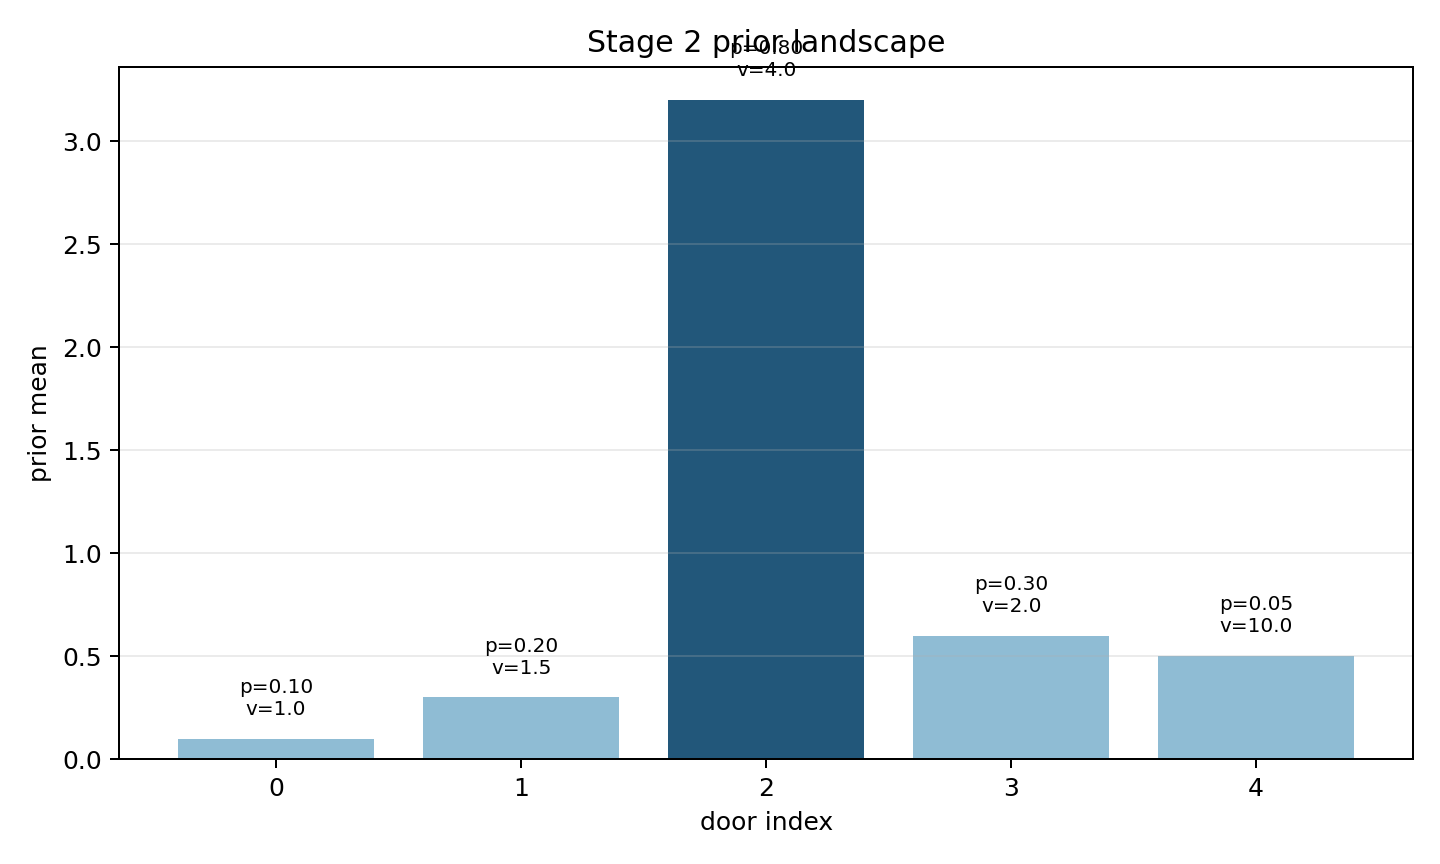
\includegraphics[width=0.85\linewidth]{../outputs/stage2_labeled_prior_landscape.png}
  \caption{Stage 2 labeled-prior landscape used in the canonical skewed
  example. The bars show prior means $\mu_j=p_jv_j$, while the annotations show
  the underlying prize probabilities and reward magnitudes.}
  \label{fig:stage2-prior-landscape}
\end{figure}

\subsection{What Stage 2 changes qualitatively}

The first qualitative change is that initial choice now matters sharply.
Figure~\ref{fig:stage2-strategy-panel} plots empirical reward against reveal
depth for all four switch rules under the neutral Monty policy
`uniform\_zero', with one panel for each initial strategy.

Three facts stand out.
\begin{itemize}
\item If the player starts at the highest-mean door, then staying is hard to
beat, because the initial pick already captures most of the prior value.
\item If the player starts randomly or at the lowest-mean door, switching
becomes attractive, and `prior\_best\_switch' can beat `uniform\_switch'.
\item `oracle\_best\_switch' remains a useful upper bound: even with labeled
priors, payoff-relevant uncertainty survives after the reveals.
\end{itemize}

\begin{figure}[t]
  \centering
  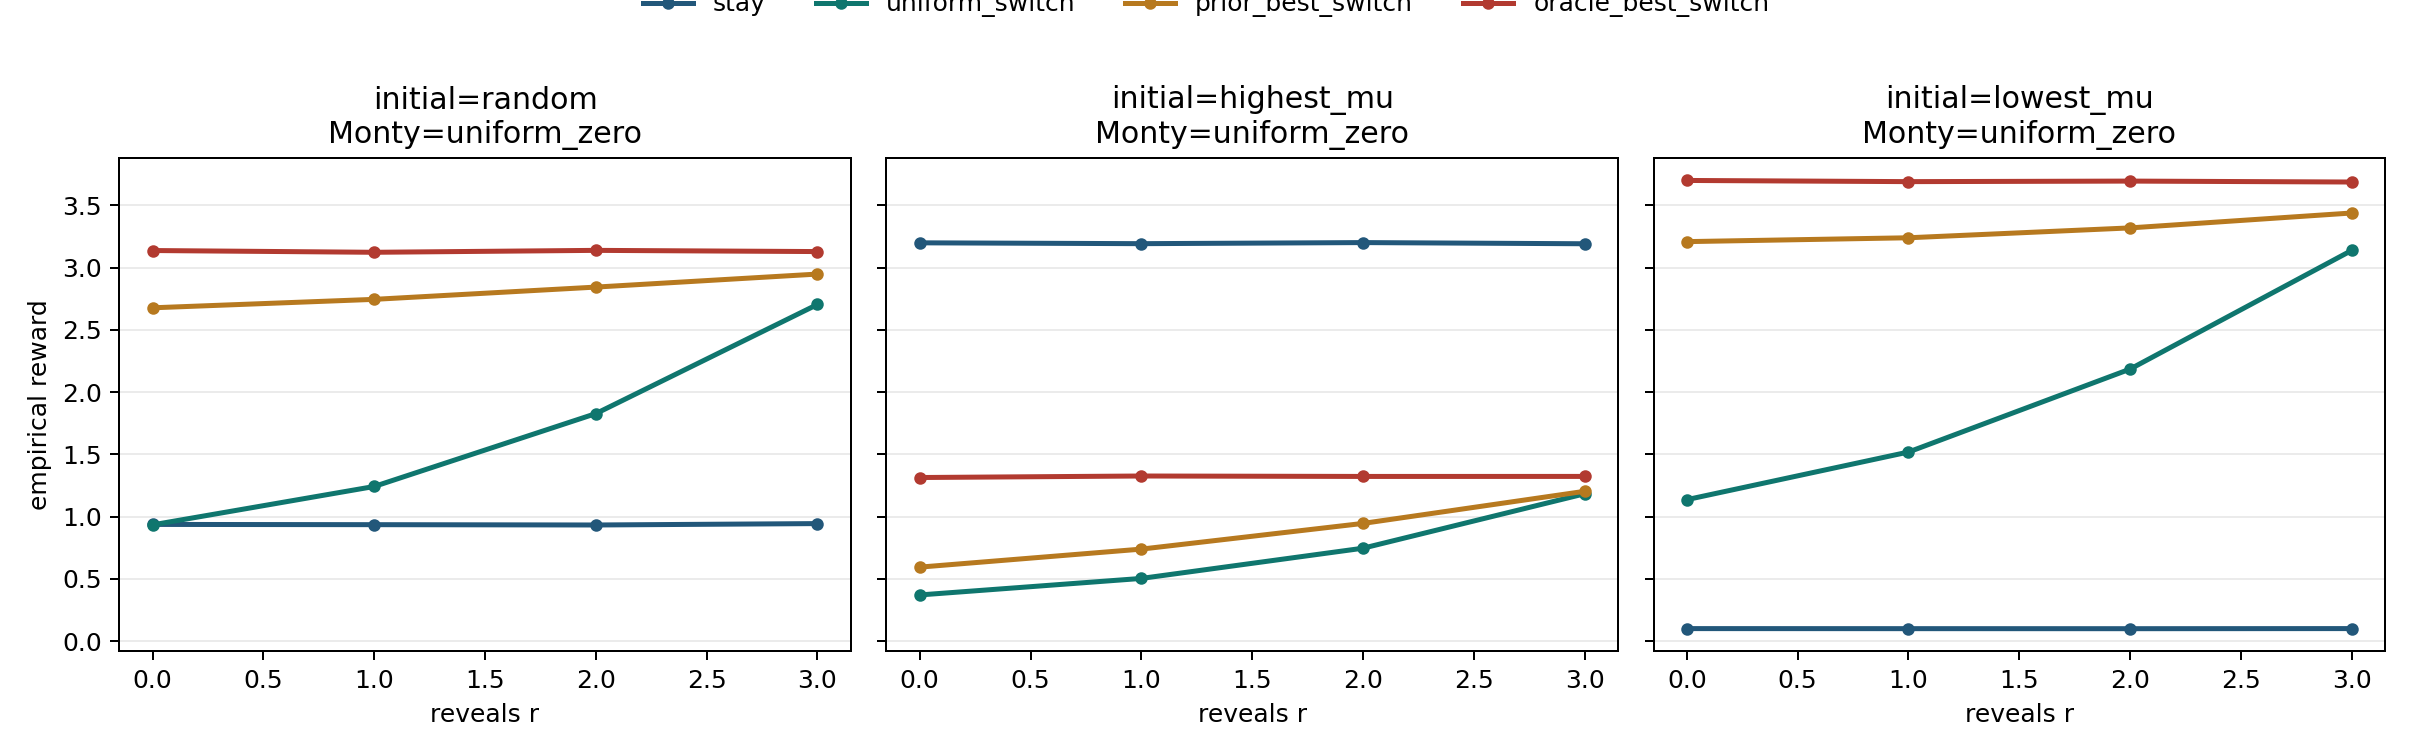
\includegraphics[width=\linewidth]{../outputs/stage2_labeled_strategy_panel.png}
  \caption{Stage 2 strategy panel under Monty=`uniform\_zero'. Once labels
  matter, the initial door and switching rule interact strongly. In this
  skewed example, `prior\_best\_switch' improves on `uniform\_switch' for
  random and low-value starts, while `stay' dominates when the player begins at
  the strongest prior-mean door.}
  \label{fig:stage2-strategy-panel}
\end{figure}

The second qualitative change is that the comparison between switching rules is
now context-dependent rather than universal. In the exchangeable model, uniform
switching was analytically forced by symmetry. In the labeled model, it becomes
just one rule among several. Sometimes it is too naive, because it ignores
useful prior structure. Sometimes it is surprisingly competitive, because the
best-looking prior-mean door is not always the door most likely to survive the
reveal process as the best remaining option.

This is precisely why the labeled model is genuinely richer than a simple
replacement of $m$ by $V$. The relevant object is no longer a scalar summary,
but a posterior landscape over surviving doors.

\subsection{Monty policy sensitivity}

Stage 2 also lets us ask whether Monty's legal reveal policy materially changes
the player's value. Figure~\ref{fig:stage2-policy-gain} summarizes the gain
\[
  \texttt{prior\_best\_switch} - \texttt{uniform\_switch}
\]
at the largest reveal depth used in the experiment, across all initial
strategies and all three Monty policies.

\begin{figure}[t]
  \centering
  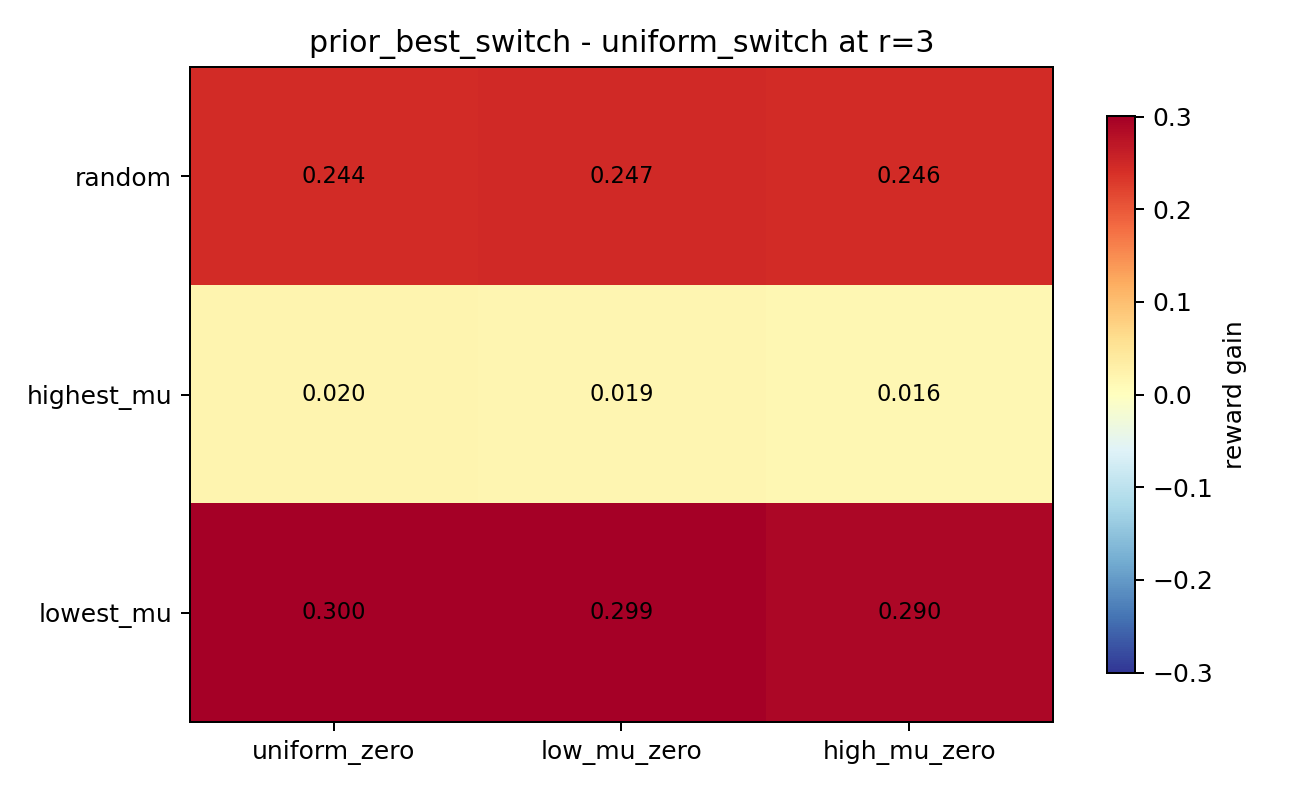
\includegraphics[width=0.88\linewidth]{../outputs/stage2_labeled_policy_gain_heatmap.png}
  \caption{Gain of `prior\_best\_switch' over `uniform\_switch' at the largest
  reveal depth in the Stage 2 run. Positive values show where label-aware
  switching beats uniform switching. The pattern depends strongly on the
  initial strategy and only weakly on Monty's reveal bias in this particular
  skewed example.}
  \label{fig:stage2-policy-gain}
\end{figure}

In this example, initial choice matters more than Monty's reveal bias: the heat
map is structured mainly by the row corresponding to the initial strategy, not
by the column corresponding to Monty's legal policy. That need not be true in
general, but it is already enough to establish the main Stage 2 point:
\begin{quote}
once doors are labeled, the decision problem is genuinely strategic, not just a
scalar reveal-depth optimization.
\end{quote}

\section{Conjectural Part IV Questions}

The next coding and theory questions should be:
\begin{enumerate}
\item In the labeled unequal-prize model, when does prior-best switching beat
uniform switching by a large margin?
\item Can low-value initial choices preserve a better switch set when there are
several high-value prize candidates rather than just one standout door?
\item How sensitive is the switch value to Monty's legal reveal policy?
\item Does a useful reduced state survive, or does the problem become genuinely
high-dimensional in the posterior reward vector?
\end{enumerate}

These are the questions that would make Part IV mathematically distinct from
Part III.

\section{Conclusion}

Multiple prizes with unequal rewards split cleanly into two regimes.

In the exchangeable regime, unequal rewards collapse to total reward mass
$V$. The theory remains scalar, and the Part I and Part II arguments survive
with only a rescaling of value. The new Stage 1 evidence shows that this is not
just a formal theorem: simulation produces the same reveal-depth curves for
very different unequal prize vectors once total reward mass is held fixed.

In the labeled regime, unequal rewards become genuinely interesting. Then the
problem is no longer about a single quantity like $t$ or $V$, but about how
posterior reward mass is distributed across doors, how Monty reveals zeros, and
how the initial choice preserves or destroys later switching opportunities.

That labeled unequal-prize regime is the natural next coding target.

\end{document}
